\chapter{Các công trình liên quan}
\label{chapter:related}
\ifpdf
    \graphicspath{{Chapter2/Chapter2Figs/PNG/}{Chapter2/Chapter2Figs/PDF/}{Chapter2/Chapter2Figs/}}
\else
    \graphicspath{{Chapter2/Chapter2Figs/EPS/}{Chapter2/Chapter2Figs/}}
\fi

\markboth{\MakeUppercase{Chương \thechapter. Các công trình liên quan}}{Chương \thechapter. Các công trình liên quan}

Trong chương này chúng tôi sẽ trình bày một cách tổng quan về các phương pháp truy vấn đối tượng trên tập dữ liệu ảnh lớn đang được sử dụng rộng rãi hiện nay. Các phương pháp cần phải thỏa hai yêu cầu là cho kết quả với độ chính xác cao và trả về trong thời gian ngắn.

Trước tiên, chúng tôi sẽ trình bày tổng quan về các thành phần của một hệ thống truy vấn ảnh cơ bản trong mục \ref{section:overall}. Mục \ref{local-features} sẽ trình bày ngắn gọn về hướng tiếp cận biểu diễn hình ảnh bằng các đặc trưng cục bộ. Nhưng khi kích cỡ của tập dữ liệu tăng thì việc so khớp các đặc trưng cục bộ tỏ ra kém hiệu quả. Trong mục \ref{bag-of-words}, chúng tôi sẽ giới thiệu mô hình Bag-of-Words (BoW) -  được ứng dụng từ lĩnh vực xử lý văn bản. Mô hình này cho thấy tính hiệu quả của nó cả về tốc độ tính toán lẫn bộ nhớ sử dụng.

Mặc dù đạt được hiệu suất cao nhưng mô hình BoW vẫn bỏ qua thông tin về không gian ảnh - một thông tin quan trọng ảnh hướng lớn đến độ chính xác của truy vấn. Trong mục \ref{spatial}, chúng tôi sẽ trình bày rõ hơn về các hướng tiếp cận dựa để khai thác được thông tin không gian ảnh, tiêu biểu là hướng tiếp cận dựa trên đặc trưng hình học và thông tin không gian của các đặc trưng cục bộ.

\section{Mô hình tổng quan}
\label{section:overall}
Mô hình tổng quan của một hệ thống truy vấn cơ bản ảnh gồm ba thành phần chính:\\
\textbf{Rút trích, biểu diễn đặc trưng ảnh.} Từ một hình ảnh, hệ thống sẽ dò tìm và phát hiện được những điểm đặc trưng, sau đó các điểm này sẽ được mô tả để rút ra được một vector tương ứng với mỗi điểm. Từ các vector đó, ta sẽ xây dựng được một histogram biểu diễn cho hình ảnh đó.\\
\textbf{So khớp các hình ảnh.} Sau khi biểu diễn các hình ảnh dưới dạng các histogram, ta tiến hành so khớp các histogram của các hình trong cơ sở dữ liệu với của hình truy vấn để tìm được những hình ảnh có độ tương đồng cao nhất so với hình ảnh truy vấn. Các hình ảnh sẽ được xếp hạng dựa trên độ tương đồng này.\\
\textbf{Hậu xử lý kết quả.} Từ danh sách có thứ tự các hình ảnh có độ tương đồng cao nhất so với hình ảnh truy vấn, ta tiến hành xử lý tùy theo mục đích cụ thể của hệ thống hoặc có thể áp dụng thêm một thuật toán để re-ranking những hình ảnh trong top đầu nhằm tăng độ chính xác.

Mô hình tổng quan của một hệ thống truy vấn ảnh cơ bản được minh họa trong hình \ref{FigOverall}.

\begin{figure}[!htbp]
  \begin{center}
    \leavevmode
    \ifpdf
      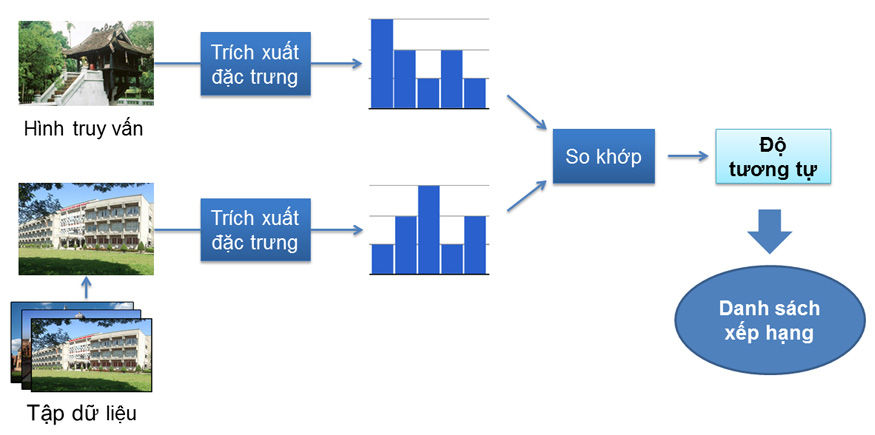
\includegraphics[scale=0.45]{overall}
    \else
      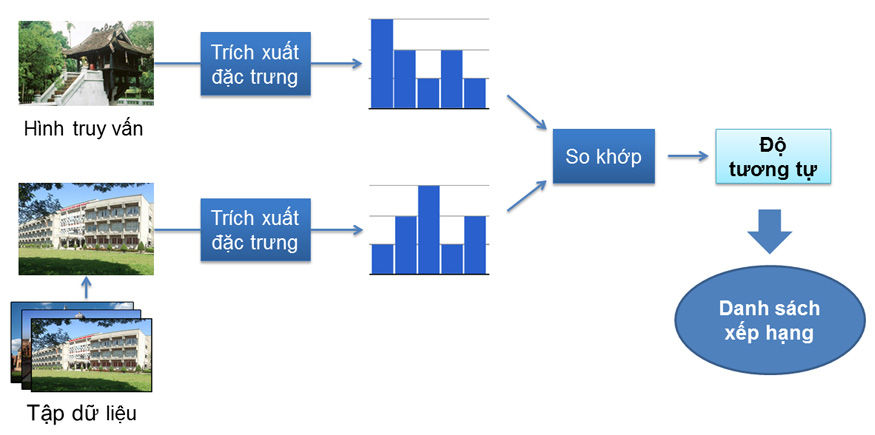
\includegraphics[scale=0.45]{overall}
    \fi
    \caption[Mô hình tổng quan của một hệ thống truy vấn ảnh]{Mô hình tổng quan của một hệ thống truy vấn ảnh.}
    \label{FigOverall}
  \end{center}
\end{figure}

\section{Biểu diễn hình ảnh bằng các đặc trưng cục bộ}
\label{local-features}

Trong lĩnh vực Thị giác Máy tính, một câu hỏi và cũng là một thách thức lớn đối với tất cả các nhà khoa học là làm sao biểu diễn được môt hình ảnh trên máy tính. Tùy theo từng mục đích cụ thể, người ta sẽ có các cách biểu diễn khác nhau. Trong truy vấn ảnh, một hình ảnh phải được biểu diễn dưới dạng sao cho bền vững trước những thay đổi như điều kiện chụp, tỉ lệ, góc chụp khác nhau hay thậm chí là những thay đổi lớn do đối tượng bị che khuất. Do sự tác động của các yếu tố này, cho dù hai hình ảnh chứa cùng một đối tượng thì vẫn có thể tồn tại một vùng hình ảnh lớn bên ngoài các đối tượng không đồng thời xuất hiện ở cả hai hình.

Để giải quyết vấn đề này, có một hướng tiếp cận phổ biến là rút trích những "chi tiết" cục bộ (local patches) trên tấm hình để biểu diễn cho hình ảnh đó. Hướng tiếp cận này được đưa ra dựa trên nhận định rằng hai hình ảnh tương tự nhau sẽ có rất nhiều những chi tiết cục bộ giống nhau và những chi tiết cục bộ này có thể được dùng để so khớp các hình ảnh với nhau. Các chi tiết này thường được rút trích bằng một trong hai phương pháp, đó là: (i) sử dụng một lưới dày đặc với nhiều mức tỉ lệ kích cỡ khác nhau (để đảm bảo bất biến về tỉ lệ) để chia hình ảnh thành nhiều chi tiết nhỏ, hoặc (ii) dùng các phương pháp dò tìm (detector) hay một kỹ thuật nào đó để lấy được các chi tiết đặc biệt (đặc trưng) trên vùng hình ảnh quan tâm và đồng thời loại bỏ những chi tiết không đảm bảo sự bất biến tỉ lệ ngay ở bước này. Có thể thấy rằng phương pháp dùng lưới để chia hình ảnh thành nhiều phần không thể áp dụng cho bài toán truy vấn ảnh với tập dữ liệu lớn vì ta cần rất nhiều không gian để lưu trữ một lượng lớn các chi tiết dày đặc với nhiều mức tỉ lệ kích cỡ khác nhau. Do vậy phương pháp biểu diễn hình ảnh bằng các đặc trưng được áp dụng cho bài toán này.

Có rất nhiều phương pháp dò tìm các điểm đặc trưng (feature detector) được đưa ra, trong đó phải kể tới các phương pháp được dùng phổ biến như Difference of Gaussians, DoG \cite{lowe2004distinctive}, Maximally Stable Extremal Regions, MSER \cite{matas2004robust} và affine invariant detector \cite{mikolajczyk2004scale}. Ngoài ra còn có các phương pháp dò tìm được xây dựng để tìm kiếm trong thời gian thực như SURF \cite{bay2006surf}, FAST \cite{rosten2010faster} và BRISK \cite{leutenegger2011brisk}.

Sau khi rút trích được các điểm đặc trưng cục bộ cho mỗi hình, dựa trên các đặc trưng đó ta sẽ quyết định xem liệu hai tấm hình bất kỳ có chứa cùng một đối tượng hay không. Để so sánh độ tương đồng của hai đặc trưng cục bộ, ta không thể dựa trên màu sắc và cường độ của chúng vì những yếu tố này không bền vững trước những thay đổi của hình ảnh. Do đó ta cần phải tìm cách lượng tử hóa độ tương đồng giữa cách đặc trưng để có thể đo được bằng các tính toán cụ thể. Trong công trình nghiên cứu nổi tiếng của Lowe \cite{lowe2004distinctive}, tác giả đã đề xuất một phương pháp để có thể tính toán được một bộ mô tả (descriptor) có tính phân loại cao và đảm bảo sự bất biến trước những thay đổi của hình ảnh, đó là SIFT descriptor. Theo sau công trình nghiên cứu này, nhiều công trình có hướng tiếp cận tương tự được đưa ra, trong đó bao gồm GLOH \cite{mikolajczyk2005performance}, SURF \cite{bay2006surf}, DAISY \cite{tola2008fast}, CONGAS \cite{zheng2009tour}, BRIEF \cite{calonder2010brief}. Đặc biệt, bằng việc đề xuất thuật toán RootSIFT được cải tiến từ SIFT, Arandjelovic và Zisserman \cite{arandjelovic2012three} đã nâng hiệu suất của phương pháp SIFT lên đáng kể. Đây cũng là phương pháp được chúng tôi chọn dùng trong hệ thống của mình.

Tóm lại, từ những bộ mô tả (descriptor) được rút trích từ tất cả các hình trong cơ sở dữ liệu và từ hình ảnh truy vấn, ta có thể tính toán được độ tương đồng giữa các hình ảnh. Tuy nhiên, hiệu suất của quá trình tính toán độ tương đồng bị giảm đi đáng kể khi thực hiện trên tập dữ liệu lớn. Trong phần tiếp theo, chúng tôi sẽ giới thiệu sơ lược về một mô hình giúp giải quyết được vấn đề này.

\section{Mô hình Bag-of-words}
\label{bag-of-words}
Mô hình BoW đã thể hiện được sức mạnh của nó trong truy vấn văn bản và được sử dụng trong các công cụ tìm kiếm văn bản mạnh mẽ như Google, Bing. Chính vì sự thành công đó, BoW đã được sử dụng trong truy vấn ảnh.

Một khó khăn lớn khi áp dụng môt hình của truy vấn văn bản vào truy vấn ảnh là trong truy vấn văn bản, một văn bản có thể dễ dàng bóc tách ra các từ trong khi đó không có cách phân chia tự nhiên nào cho các hình ảnh. Như đã giới thiệu trong mục \ref{local-features}, một hình ảnh hoàn toàn có thể chia thành các đặc trưng cục bộ, tuy nhiên các đặc trưng này lại hoàn toàn phân biệt với nhau, vậy làm thế nào để xây dựng được các \textit{từ} từ các đặc trưng này?

Nghiên cứu của Sivic và Zisserman \cite{sivic2003video} là công trình đầu tiên ứng dụng hướng tiếp cận của truy vấn văn bản vào truy vấn ảnh\footnote{Mục đích của tác giả trong nghiên cứu này là truy vấn trên video nhưng ta hoàn toàn có thể chuyển sang bài toán truy vấn ảnh bằng cách rút trích các frame trong video theo từng giây}. Trong công trình này tác giả đã giới thiệu khái niệm visual word, được tạo ra bằng cách sử dụng thuật toán gom cụm K-Means để gom cụm các đặc trưng cục bộ. Hình \ref{FigVisualWords} cho thấy một vài ví dụ về các visual word. Tương tự như trong truy vấn văn bản, hình ảnh sẽ được rút trích các đặc trưng cục bộ rồi tiến hành gom cụm để biểu diễn thành các visual word, sau đó được đánh trọng số bằng tf-idf\cite{manning2008introduction}, rồi biểu diễn dưới dạng mô hình BoW và sử dụng chỉ mục ngược để tăng hiệu suất cho quá trình truy vấn. Thí nghiệm được tiến hành trên 4000 ảnh (frame) được lấy từ video và rút trích được 10,000 visual word từ những hình ảnh đó.

\begin{figure}[!htbp]
  \begin{center}
    \leavevmode
    \ifpdf
      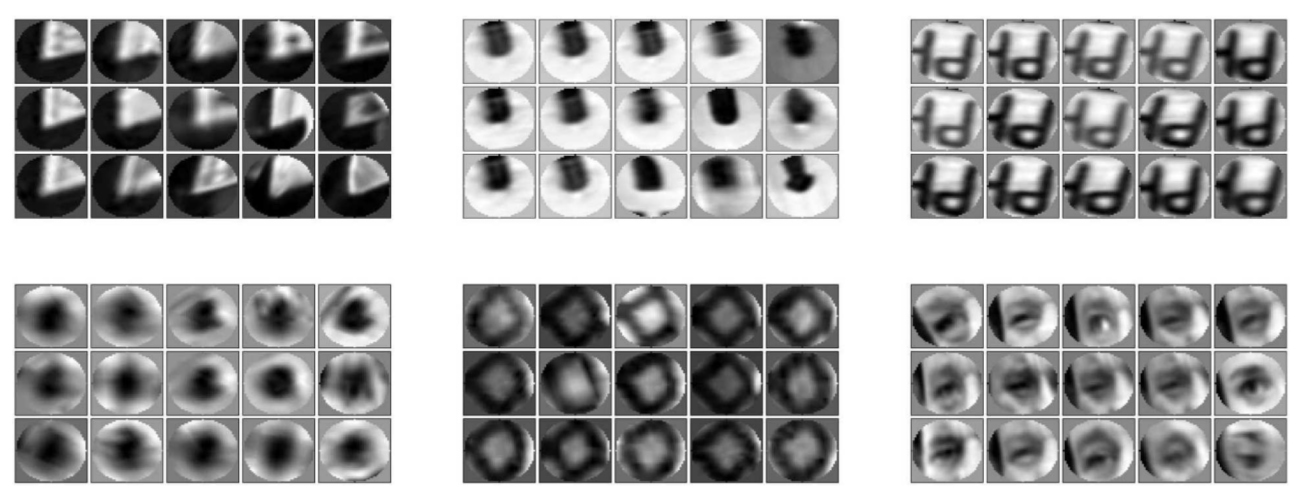
\includegraphics[scale=0.32]{visualWords}
    \else
      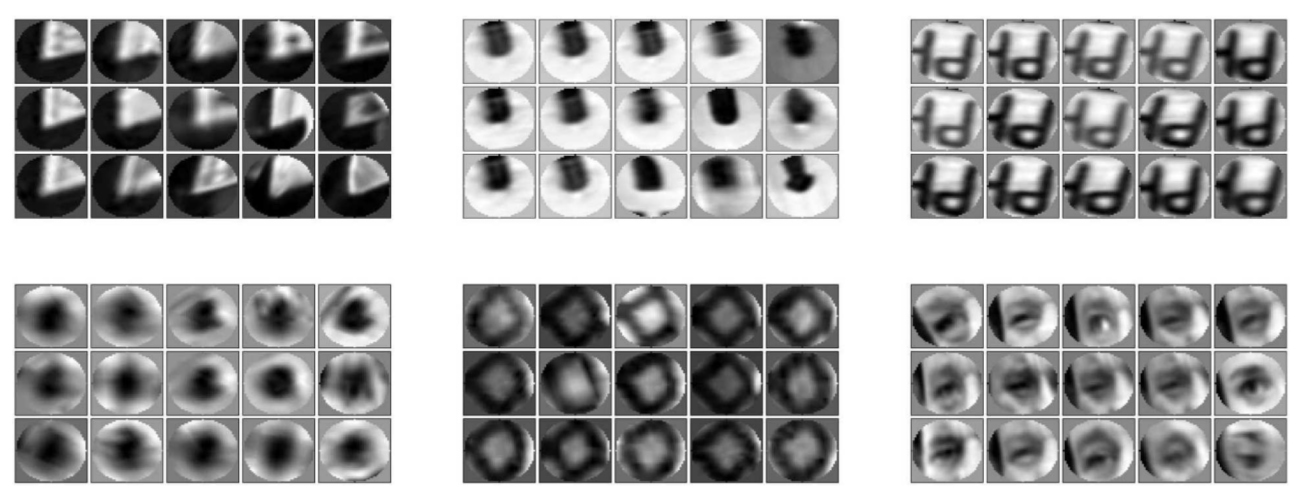
\includegraphics[scale=0.32]{visualWords}
    \fi
    \caption[Các từ visual word]{\textbf{Các visual word.} Mỗi nhóm là một nhóm các đặc trưng cục bộ được rút trích từ hình ảnh, gom vào cùng một cụm và cùng được biểu diễn bằng một visual word. Hình ảnh được lấy từ bài báo \cite{sivic2009efficient}.}
    \label{FigVisualWords}
  \end{center}
\end{figure}
Trong thực tế, để truy vấn ảnh trên những tập dữ liệu lớn, để cho kết quả tốt thì số lượng visual word không thể vào khoảng 10,000 từ như trong thí nghiệm của Sivic và Zisserman \cite{sivic2003video} mà phải lên tới hàng triệu từ\cite{philbin2007object}. Trong khi đó, độ phức tạp của thuật toán K-Means là \textit{O(N\textsubscript{w}N\textsubscript{d})} với N\textsubscript{w}, N\textsubscript{d} lần lượt là kích cỡ của visual word và số tập của bộ mô tả huấn luyện (training descriptor set). Trên những tập dữ liệu lớn thì N\textsubscript{d} $\geq$ N\textsubscript{w} nên độ phức tạp luôn lớn hơn $O(N^2_w)$. Do đó nếu dùng K-Means cho bài toán này chi phí tính tính toán sẽ vô cùng lớn. Nister và Stewenius \cite{nister2006scalable} đã đề xuất phương pháp giải quyết cho bài toán này bằng cách xây dựng một cây từ vựng mà về bản chất thì nó chính là thuật toán Hierarchical K-Means (HKM). Để minh họa cho thuật toán này, tác giả đã cho thử nghiệm trên bộ ảnh gồm 1 triệu hình ảnh. Không lâu sau đó, Philbin và các đồng nghiệp \cite{philbin2007object} đã đề xuất một hướng tiếp cận khác dựa trên thuật toán \textit{xấp xỉ K-Means}, Approximate K-Means (AKM). Tác giả cũng cho chạy thử nghiệm AKM trên 16.7 triệu đặc trưng để gom cụm thành 1 triệu từ. Các thí nghiệm cho thấy rằng, khi so sánh AKM với K-Means thì về độ chính xác thì AKM xấp xỉ K-Means tuy nhiên chi phí tính toán chỉ bằng một phần nhỏ của K-Means. Còn khi so sánh AKM với HKM thì AKM không những vượt xa về độ chính xác mà còn có thể áp dụng cho những tập dữ liệu lớn. Chi phí tính toán của cả HKM và AKM đều là $O(N_d log(N_w))$.

\section{Sử dụng thông tin không gian ảnh trong truy vấn ảnh}
\label{spatial}

Mặc dù đạt được những kết quả rất đáng chú ý nhưng mô hình cơ bản của BoW vẫn bị giới hạn về độ chính xác do bỏ qua một thông tin quan trọng, đó là sự phân bố về không gian của các visual word. Do đó các đặc trưng cục bộ được xử lý một cách rời rạc, không liên quan tới nhau. Hình \ref{FigLimited} minh họa cho trường hợp các ảnh khác nhau có cùng biểu diễn BoW giống nhau nếu không xem xét sự phân bố về không gian của các visual word.
\begin{figure}[!htbp]
  \begin{center}
    \leavevmode
    \ifpdf
      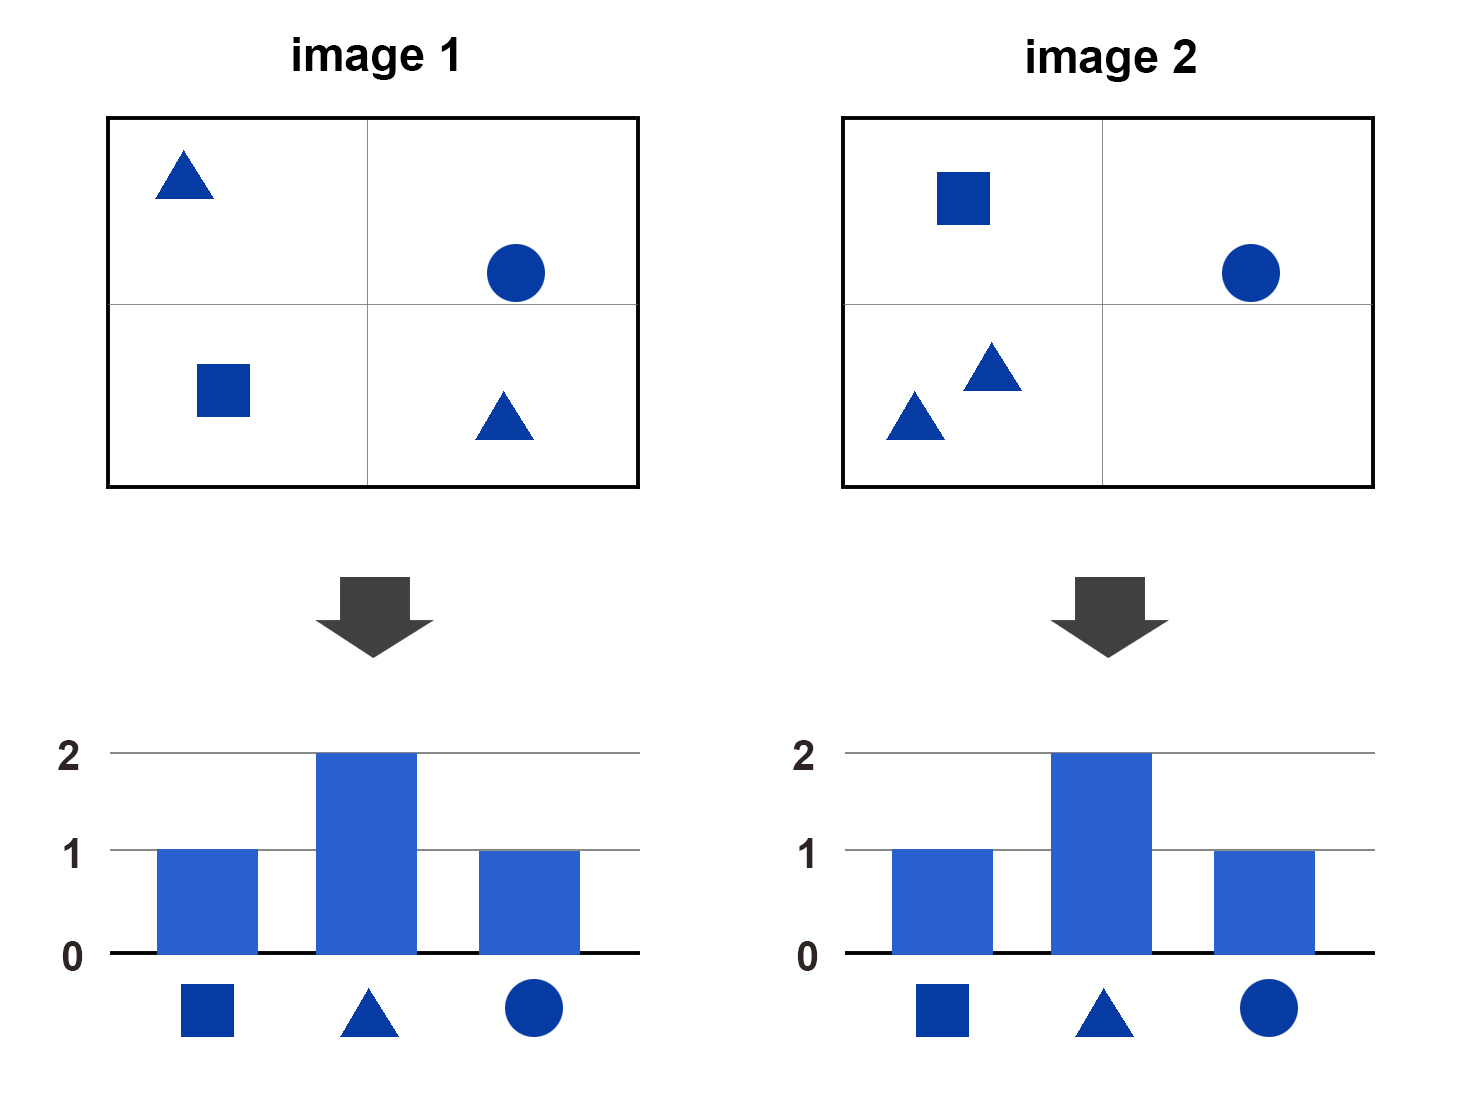
\includegraphics[scale=0.25]{limited}
    \else
      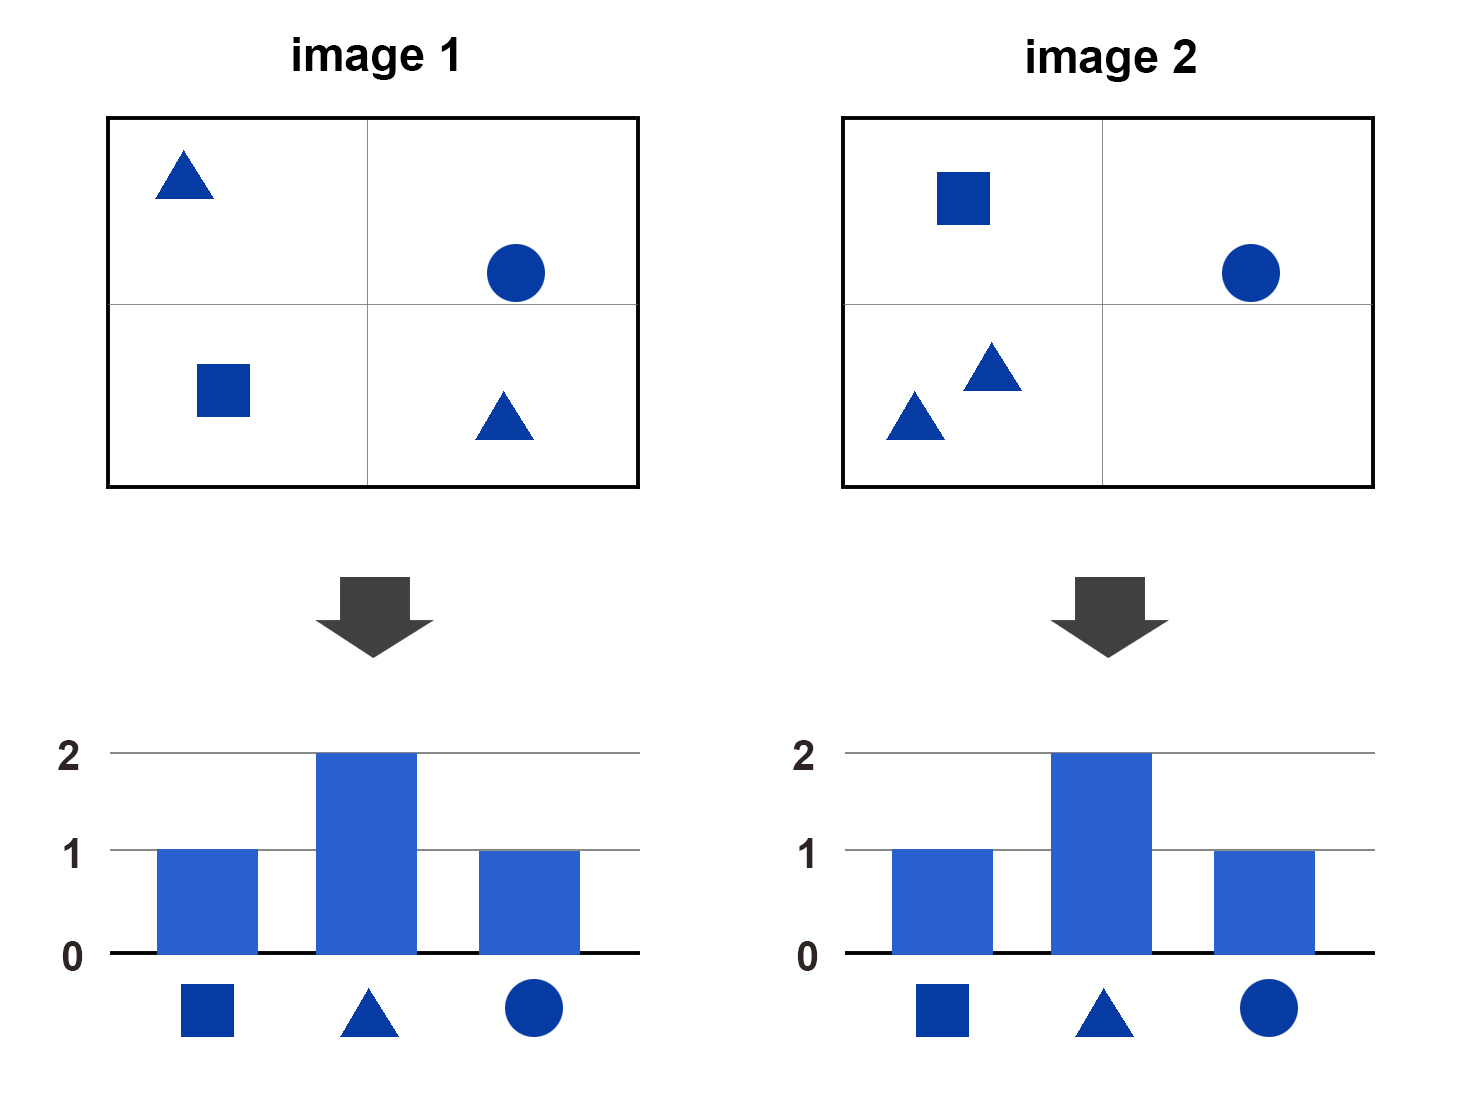
\includegraphics[scale=0.25]{limited}
    \fi
    \caption[Bỏ qua thông tin về sự phân bố trong không gian của các visual word trong mô hình BoW]{\textbf{Bỏ qua thông tin về sự phân bố trong không gian của các visual word trong mô hình BoW.} Nếu bỏ qua thông tin về sự phân bố trong không gian của các visual word, hai hình ảnh trên sẽ được biểu diễn dưới dạng biểu đồ giống nhau do đó chúng sẽ được xem như hai hình ảnh giống nhau. Trong khi đó hình ảnh $I_1$ hoàn toàn khác với $I_2$.}
    \label{FigLimited}
  \end{center}
\end{figure}

Để giải quyết vấn đề trên, rất nhiều công trình nghiên cứu đã được đưa ra. Phần lớn các hướng tiếp cận được chia ra làm hai dạng là tiếp cận dựa trên đặc trưng hình học và tiếp cận dựa trên thông tin không gian của các điểm đặc trưng cục bộ. Mục \ref{geometry} chúng tôi sẽ trình bày về các phương pháp dựa trên đặc trưng hình học. Hướng tiếp cận còn lại sẽ được trình bày chi tiết ở mục \ref{spm}.

\subsection{Các hướng tiếp cận dựa trên đặc trưng hình học}
\label{geometry}
Các phương pháp sử dụng đặc trưng hình học để so khớp thường được dùng ở bước hậu xử lý để nhận dạng hình học. Dưới đây là một vài công trình tiêu biểu sử dụng hướng tiếp cận này.

Sivic và Zisserman \cite{sivic2003video} đã đo đạc sự nhất quán không gian cục bộ (local spatial consistency) trong các so khớp giữa hình ảnh truy vấn và từng hình ảnh trong cơ sở dữ liệu từ đó tái xếp hạng lại danh sách kết quả trả về. Việc đo đạc sự nhất quán không gian cục bộ trong so khớp hình ảnh cũng được đề cập tới trước đó trong các công trình như \cite{zhang1995robust} và \cite{schmid1997local}.

Trong một công trình nghiên cứu \cite{philbin2007object}, tác giả sử dụng thuật toán RANSAC \cite{fischler1981random} để kiểm tra sự nhất quán hình học giữa các đặc trưng cục bộ trùng khớp. RANSAC là một trong những phương pháp phổ biến nhất cho hậu xử lý toàn cục trên hình ảnh. Đặc biệt, trong một công trình khác, Zhang và các đồng nghiệp \cite{zhang2011image} đề xuất mã hóa thông tin không gian ảnh qua các mệnh đề trực quan hình học (GVP) kết hợp với RANSAC đã cho kết quả rất đáng chú ý với bộ dữ liệu lên tới hàng triệu ảnh.

Trong khi đó, công trình \cite{lin2010local} và \cite{lampert2009detecting} lại xếp hạng các hình ảnh dựa trên điểm số so khớp của hình ảnh truy vấn với những cửa sổ con được định vị trên hình. Phương pháp này mã hóa được nhiều thông tin không gian ảnh hơn so với mô hình BoW trên toàn bộ tấm hình và giúp định vị hình ảnh truy vấn.

Nhìn chung, những phương pháp sử dụng hướng tiếp cận hình học đều cho kết quả tốt. Tuy nhiên, khi vùng truy vấn lớn hơn thì chúng chỉ được dùng để tái xếp hạng một số lượng giới hạn ở các hình ảnh ở top đầu của kết quả trả về vì vấn đề về chi phí cho bộ nhớ và tốc độ thực hiện.

\subsection{Các hướng tiếp cận dựa trên thông tin không gian của các điểm đặc trưng cục bộ}
\label{spm}

Hướng tiếp cận dựa trên đặc trưng hình học là hướng tiếp cận mang tính toàn cục, tức là xem xét đối tượng dưới một cái nhìn tổng quan, toàn thể chứ không xem xét chi tiết những thành phần cấu thành nó. Hướng tiếp cận dựa trên các đặc trưng cục bộ lại ngược lại, xem đối tượng là một tập hợp của nhiều thành phần và dựa trên những thành phần đó để xác định đối tượng. Lazebnik \cite{lazebnik2006beyond} đã giới thiệu một phương pháp nền tảng, được bắt nguồn từ ý tưởng \textit{so khớp phân cấp} (pyramid matching) của Grauman và Darrell \cite{grauman2005pyramid}, đó là phương pháp \textit{so khớp không gian phân cấp} (Spatial Pyramid Matching - SPM). Ý tưởng của phương pháp này là lặp đi lặp lại việc chia nhỏ hình ảnh và tính toán biểu đồ của các đặc trưng cục bộ với mức độ chi tiết tăng dần. SPM đã giúp nâng cao một cách đáng kể độ chính xác cho mô hình BoW và tỏ ra là một phương pháp đơn giản nhưng hiệu quả. Mặc dù vậy, SPM cũng làm tăng thời gian thực hiện truy vấn bởi khi mức độ chi tiết càng cao thì kích cỡ biểu đồ của các đặc trưng cục bộ cũng tăng theo làm tăng chi phí tính toán trong quá trình so khớp, vì vậy SPM vẫn chưa thích hợp cho các bài toán yêu cầu thời gian thực.

\section{Kết chương}

Việc biểu diễn hình ảnh bằng các đặc trưng cục bộ đã đặt nền tảng cho việc đưa ra các phương pháp để truy vấn đối tượng trên ảnh. Mô hình BoW đã chứng minh tính hiệu quả của mình trong truy vấn ảnh và việc kết hợp phương pháp chỉ mục ngược (inverted index) giúp giảm đáng kể thời gian thực hiện truy vấn. Tuy nhiên, mô hình BoW vẫn bị giới hạn về độ chính xác do bỏ qua thông tin không gian ảnh. Trong khi đó, rất nhiều hướng tiếp cận khác tận dụng được thông tin này đã nâng độ chính xác truy vấn nhưng lại cần chi phí tính toán cao, tốc độ phản hồi chậm.

Phương pháp chúng tôi đề xuất tập trung vào việc cân bằng độ chính xác truy vấn và tốc độ. Để đạt được mục đích đó, chi phí bộ nhớ cao có thể được chấp nhận.

